
%% bare_jrnl.tex
%% V1.4
%% 2012/12/27
%% by Michael Shell
%% see http://www.michaelshell.org/
%% for current contact information.
%%
%% This is a skeleton file demonstrating the use of IEEEtran.cls
%% (requires IEEEtran.cls version 1.8 or later) with an IEEE journal paper.
%%
%% Support sites:
%% http://www.michaelshell.org/tex/ieeetran/
%% http://www.ctan.org/tex-archive/macros/latex/contrib/IEEEtran/
%% and
%% http://www.ieee.org/



% *** Authors should verify (and, if needed, correct) their LaTeX system  ***
% *** with the testflow diagnostic prior to trusting their LaTeX platform ***
% *** with production work. IEEE's font choices can trigger bugs that do  ***
% *** not appear when using other class files.                            ***
% The testflow support page is at:
% http://www.michaelshell.org/tex/testflow/


%%*************************************************************************
%% Legal Notice:
%% This code is offered as-is without any warranty either expressed or
%% implied; without even the implied warranty of MERCHANTABILITY or
%% FITNESS FOR A PARTICULAR PURPOSE! 
%% User assumes all risk.
%% In no event shall IEEE or any contributor to this code be liable for
%% any damages or losses, including, but not limited to, incidental,
%% consequential, or any other damages, resulting from the use or misuse
%% of any information contained here.
%%
%% All comments are the opinions of their respective authors and are not
%% necessarily endorsed by the IEEE.
%%
%% This work is distributed un-Americander the LaTeX Project Public License (LPPL)
%% ( http://www.latex-project.org/ ) version 1.3, and may be freely used,
%% distributed and modified. A copy of the LPPL, version 1.3, is included
%% in the base LaTeX documentation of all distributions of LaTeX released
%% 2003/12/01 or later.
%% Retain all contribution notices and credits.
%% ** Modified files should be clearly indicated as such, including  **
%% ** renaming them and changing author support contact information. **
%%
%% File list of work: IEEEtran.cls, IEEEtran_HOWTO.pdf, bare_adv.tex,
%%                    bare_conf.tex, bare_jrnl.tex, bare_jrnl_compsoc.tex,
%%                    bare_jrnl_transmag.tex
%%*************************************************************************

% Note that the a4paper option is mainly intended so that authors in
% countries using A4 can easily print to A4 and see how their papers will
% look in print - the typesetting of the document will not typically be
% affected with changes in paper size (but the bottom and side margins will).
% Use the testflow package mentioned above to verify correct handling of
% both paper sizes by the user's LaTeX system.
%
% Also note that the "draftcls" or "draftclsnofoot", not "draft", option
% should be used if it is desired that the figures are to be displayed in
% draft mode.
%
\documentclass[journal,twoside,11pt]{IEEEtran}
%
% If IEEEtran.cls has not been installed into the LaTeX system files,
% manually specify the path to it like:
% \documentclass[journal]{../sty/IEEEtran}
%some macro
\newcommand{\mbf}{\mathbf}
\newcommand{\wtd}{\widetilde}

\usepackage[ruled]{algorithm2e}
\usepackage{url}
\usepackage{multirow}
%\usepackage{cite}
\usepackage{graphicx}
\usepackage{amssymb}
\usepackage{amsmath}
\usepackage{amsfonts}
\usepackage{color}
\usepackage{epstopdf}
\usepackage{verbatim} 
\usepackage[center]{caption}



%\usepackage{subcaption}
\usepackage{listings}
\usepackage{xcolor}

\lstset{ %
    backgroundcolor=\color{white},   % choose the background color; you must add \usepackage{color} or \usepackage{xcolor}
    basicstyle=\footnotesize,        % the size of the fonts that are used for the code
	breakatwhitespace=false,         % sets if automatic breaks should only happen at whitespace
	 breaklines=true,                 % sets automatic line breaking
	captionpos=b,                    % sets the caption-position to bottom
	commentstyle=\color{mygreen},    % comment style
	deletekeywords={...},            % if you want to delete keywords from the given language
	escapeinside={\%*}{*)},          % if you want to add LaTeX within your code
	extendedchars=true,              % lets you use non-ASCII characters; for 8-bits encodings only, does not work with UTF-8
	%frame=single,                    % adds a frame around the code
	keepspaces=true,                 % keeps spaces in text, useful for keeping indentation of code (possibly needs columns=flexible)
	keywordstyle=\color{blue},       % keyword style
	language=Octave,                 % the language of the code
	morekeywords={*,...},            % if you want to add more keywords to the set
	%numbers=left,                    % where to put the line-numbers; possible values are (none, left, right)
	%numbersep=5pt,                   % how far the line-numbers are from the code
	%numberstyle=\tiny\color{mygray}, % the style that is used for the line-numbers
	rulecolor=\color{black},         % if not set, the frame-color may be changed on line-breaks within not-black text (e.g. comments (green here))
	showspaces=false,                % show spaces everywhere adding particular underscores; it overrides 'showstringspaces'
	showstringspaces=false,          % underline spaces within strings only
	showtabs=false,                  % show tabs within strings adding particular underscores
	stepnumber=2,                    % the step between two line-numbers. If it's 1, each line will be numbered
	stringstyle=\color{mymauve},     % string literal style
	tabsize=1,                       % sets default tabsize to 2 spaces
	title=\lstname                   % show the filename of files included with \lstinputlisting; also try caption instead of title
}

\lstdefinestyle{customc}{
         belowcaptionskip=-1\baselineskip,
	breaklines=true,
	%frame=L,
	xleftmargin=\parindent,
	language=C++,
	showstringspaces=false,
	basicstyle=\footnotesize\ttfamily,
	keywordstyle=\bfseries\color{green!40!black},
	commentstyle=\itshape\color{purple!40!black},
	identifierstyle=\color{blue},
	stringstyle=\color{orange},
}

\lstdefinestyle{customasm}{
    belowcaptionskip=1\baselineskip,
	%frame=L,
	xleftmargin=\parindent,
	language=[x86masm]Assembler,
	basicstyle=\footnotesize\ttfamily,
	commentstyle=\itshape\color{purple!40!black},
}

\lstset{escapechar=@,style=customc}
\newtheorem{lemma}{Lemma}






% Some very useful LaTeX packages include:
% (uncomment the ones you want to load)


% *** MISC UTILITY PACKAGES ***
%
%\usepackage{ifpdf}
% Heiko Oberdiek's ifpdf.sty is very useful if you need conditional
% compilation based on whether the output is pdf or dvi.
% usage:
% \ifpdf
%   % pdf code
% \else
%   % dvi code
% \fi
% The latest version of ifpdf.sty can be obtained from:
% http://www.ctan.org/tex-archive/macros/latex/contrib/oberdiek/
% Also, note that IEEEtran.cls V1.7 and later provides a builtin
% \ifCLASSINFOpdf conditional that works the same way.
% When switching from latex to pdflatex and vice-versa, the compiler may
% have to be run twice to clear warning/error messages.






% *** CITATION PACKAGES ***
%
%\usepackage{cite}
% cite.sty was written by Donald Arseneau
% V1.6 and later of IEEEtran pre-defines the format of the cite.sty package
% \cite{} output to follow that of IEEE. Loading the cite package will
% result in citation numbers being automatically sorted and properly
% "compressed/ranged". e.g., [1], [9], [2], [7], [5], [6] without using
% cite.sty will become [1], [2], [5]--[7], [9] using cite.sty. cite.sty's
% \cite will automatically add leading space, if needed. Use cite.sty's
% noadjust option (cite.sty V3.8 and later) if you want to turn this off
% such as if a citation ever needs to be enclosed in parenthesis.
% cite.sty is already installed on most LaTeX systems. Be sure and use
% version 4.0 (2003-05-27) and later if using hyperref.sty. cite.sty does
% not currently provide for hyperlinked citations.
% The latest version can be obtained at:
% http://www.ctan.org/tex-archive/macros/latex/contrib/cite/
% The documentation is contained in the cite.sty file itself.






% *** GRAPHICS RELATED PACKAGES ***
%
\ifCLASSINFOpdf
  % \usepackage[pdftex]{graphicx}
  % declare the path(s) where your graphic files are
  % \graphicspath{{../pdf/}{../jpeg/}}
  % and their extensions so you won't have to specify these with
  % every instance of \includegraphics
  % \DeclareGraphicsExtensions{.pdf,.jpeg,.png}
\else
  % or other class option (dvipsone, dvipdf, if not using dvips). graphicx
  % will default to the driver specified in the system graphics.cfg if no
  % driver is specified.
  % \usepackage[dvips]{graphicx}
  % declare the path(s) where your graphic files are
  % \graphicspath{{../eps/}}
  % and their extensions so you won't have to specify these with
  % every instance of \includegraphics
  % \DeclareGraphicsExtensions{.eps}
\fi
% graphicx was written by David Carlisle and Sebastian Rahtz. It is
% required if you want graphics, photos, etc. graphicx.sty is already
% installed on most LaTeX systems. The latest version and documentation
% can be obtained at: 
% http://www.ctan.org/tex-archive/macros/latex/required/graphics/
% Another good source of documentation is "Using Imported Graphics in
% LaTeX2e" by Keith Reckdahl which can be found at:
% http://www.ctan.org/tex-archive/info/epslatex/
%
% latex, and pdflatex in dvi mode, support graphics in encapsulated
% postscript (.eps) format. pdflatex in pdf mode supports graphics
% in .pdf, .jpeg, .png and .mps (metapost) formats. Users should ensure
% that all non-photo figures use a vector format (.eps, .pdf, .mps) and
% not a bitmapped formats (.jpeg, .png). IEEE frowns on bitmapped formats
% which can result in "jaggedy"/blurry rendering of lines and letters as
% well as large increases in file sizes.
%
% You can find documentation about the pdfTeX application at:
% http://www.tug.org/applications/pdftex





% *** MATH PACKAGES ***
%
%\usepackage[cmex10]{amsmath}
% A popular package from the American Mathematical Society that provides
% many useful and powerful commands for dealing with mathematics. If using
% it, be sure to load this package with the cmex10 option to ensure that
% only type 1 fonts will utilized at all point sizes. Without this option,
% it is possible that some math symbols, particularly those within
% footnotes, will be rendered in bitmap form which will result in a
% document that can not be IEEE Xplore compliant!
%
% Also, note that the amsmath package sets \interdisplaylinepenalty to 10000
% thus preventing page breaks from occurring within multiline equations. Use:
%\interdisplaylinepenalty=2500
% after loading amsmath to restore such page breaks as IEEEtran.cls normally
% does. amsmath.sty is already installed on most LaTeX systems. The latest
% version and documentation can be obtained at:
% http://www.ctan.org/tex-archive/macros/latex/required/amslatex/math/





% *** SPECIALIZED LIST PACKAGES ***
%
%\usepackage{algorithmic}
% algorithmic.sty was written by Peter Williams and Rogerio Brito.
% This package provides an algorithmic environment fo describing algorithms.
% You can use the algorithmic environment in-text or within a figure
% environment to provide for a floating algorithm. Do NOT use the algorithm
% floating environment provided by algorithm.sty (by the same authors) or
% algorithm2e.sty (by Christophe Fiorio) as IEEE does not use dedicated
% algorithm float types and packages that provide these will not provide
% correct IEEE style captions. The latest version and documentation of
% algorithmic.sty can be obtained at:
% http://www.ctan.org/tex-archive/macros/latex/contrib/algorithms/
% There is also a support site at:
% http://algorithms.berlios.de/index.html
% Also of interest may be the (relatively newer and more customizable)
% algorithmicx.sty package by Szasz Janos:
% http://www.ctan.org/tex-archive/macros/latex/contrib/algorithmicx/




% *** ALIGNMENT PACKAGES ***
%
%\usepackage{array}
% Frank Mittelbach's and David Carlisle's array.sty patches and improves
% the standard LaTeX2e array and tabular environments to provide better
% appearance and additional user controls. As the default LaTeX2e table
% generation code is lacking to the point of almost being broken with
% respect to the quality of the end results, all users are strongly
% advised to use an enhanced (at the very least that provided by array.sty)
% set of table tools. array.sty is already installed on most systems. The
% latest version and documentation can be obtained at:
% http://www.ctan.org/tex-archive/macros/latex/required/tools/


% IEEEtran contains the IEEEeqnarray family of commands that can be used to
% generate multiline equations as well as matrices, tables, etc., of high
% quality.




% *** SUBFIGURE PACKAGES ***
%\ifCLASSOPTIONcompsoc
%  \usepackage[caption=false,font=normalsize,labelfont=sf,textfont=sf]{subfig}
%\else
%  \usepackage[caption=false,font=footnotesize]{subfig}
%\fi
% subfig.sty, written by Steven Douglas Cochran, is the modern replacement
% for subfigure.sty, the latter of which is no longer maintained and is
% incompatible with some LaTeX packages including fixltx2e. However,
% subfig.sty requires and automatically loads Axel Sommerfeldt's caption.sty
% which will override IEEEtran.cls' handling of captions and this will result
% in non-IEEE style figure/table captions. To prevent this problem, be sure
% and invoke subfig.sty's "caption=false" package option (available since
% subfig.sty version 1.3, 2005/06/28) as this is will preserve IEEEtran.cls
% handling of captions.
% Note that the Computer Society format requires a larger sans serif font
% than the serif footnote size font used in traditional IEEE formatting
% and thus the need to invoke different subfig.sty package options depending
% on whether compsoc mode has been enabled.
%
% The latest version and documentation of subfig.sty can be obtained at:
% http://www.ctan.org/tex-archive/macros/latex/contrib/subfig/




% *** FLOAT PACKAGES ***
%
%\usepackage{fixltx2e}
% fixltx2e, the successor to the earlier fix2col.sty, was written by
% Frank Mittelbach and David Carlisle. This package corrects a few problems
% in the LaTeX2e kernel, the most notable of which is that in current
% LaTeX2e releases, the ordering of single and double column floats is not
% guaranteed to be preserved. Thus, an unpatched LaTeX2e can allow a
% single column figure to be placed prior to an earlier double column
% figure. The latest version and documentation can be found at:
% http://www.ctan.org/tex-archive/macros/latex/base/


%\usepackage{stfloats}
% stfloats.sty was written by Sigitas Tolusis. This package gives LaTeX2e
% the ability to do double column floats at the bottom of the page as well
% as the top. (e.g., "\begin{figure*}[!b]" is not normally possible in
% LaTeX2e). It also provides a command:
%\fnbelowfloat
% to enable the placement of footnotes below bottom floats (the standard
% LaTeX2e kernel puts them above bottom floats). This is an invasive package
% which rewrites many portions of the LaTeX2e float routines. It may not work
% with other packages that modify the LaTeX2e float routines. The latest
% version and documentation can be obtained at:
% http://www.ctan.org/tex-archive/macros/latex/contrib/sttools/
% Do not use the stfloats baselinefloat ability as IEEE does not allow
% \baselineskip to stretch. Authors submitting work to the IEEE should note
% that IEEE rarely uses double column equations and that authors should try
% to avoid such use. Do not be tempted to use the cuted.sty or midfloat.sty
% packages (also by Sigitas Tolusis) as IEEE does not format its papers in
% such ways.
% Do not attempt to use stfloats with fixltx2e as they are incompatible.
% Instead, use Morten Hogholm'a dblfloatfix which combines the features
% of both fixltx2e and stfloats:
%
% \usepackage{dblfloatfix}
% The latest version can be found at:
% http://www.ctan.org/tex-archive/macros/latex/contrib/dblfloatfix/




%\ifCLASSOPTIONcaptionsoff
%  \usepackage[nomarkers]{endfloat}
% \let\MYoriglatexcaption\caption
% \renewcommand{\caption}[2][\relax]{\MYoriglatexcaption[#2]{#2}}
%\fi
% endfloat.sty was written by James Darrell McCauley, Jeff Goldberg and 
% Axel Sommerfeldt. This package may be useful when used in conjunction with 
% IEEEtran.cls'  captionsoff option. Some IEEE journals/societies require that
% submissions have lists of figures/tables at the end of the paper and that
% figures/tables without any captions are placed on a page by themselves at
% the end of the document. If needed, the draftcls IEEEtran class option or
% \CLASSINPUTbaselinestretch interface can be used to increase the line
% spacing as well. Be sure and use the nomarkers option of endfloat to
% prevent endfloat from "marking" where the figures would have been placed
% in the text. The two hack lines of code above are a slight modification of
% that suggested by in the endfloat docs (section 8.4.1) to ensure that
% the full captions always appear in the list of figures/tables - even if
% the user used the short optional argument of \caption[]{}.
% IEEE papers do not typically make use of \caption[]'s optional argument,
% so this should not be an issue. A similar trick can be used to disable
% captions of packages such as subfig.sty that lack options to turn off
% the subcaptions:
% For subfig.sty:
% \let\MYorigsubfloat\subfloat
% \renewcommand{\subfloat}[2][\relax]{\MYorigsubfloat[]{#2}}
% However, the above trick will not work if both optional arguments of
% the \subfloat command are used. Furthermore, there needs to be a
% description of each subfigure *somewhere* and endfloat does not add
% subfigure captions to its list of figures. Thus, the best approach is to
% avoid the use of subfigure captions (many IEEE journals avoid them anyway)
% and instead reference/explain all the subfigures within the main caption.
% The latest version of endfloat.sty and its documentation can obtained at:
% http://www.ctan.org/tex-archive/macros/latex/contrib/endfloat/
%
% The IEEEtran \ifCLASSOPTIONcaptionsoff conditional can also be used
% later in the document, say, to conditionally put the References on a 
% page by themselves.




% *** PDF, URL AND HYPERLINK PACKAGES ***
%
%\usepackage{url}
% url.sty was written by Donald Arseneau. It provides better support for
% handling and breaking URLs. url.sty is already installed on most LaTeX
% systems. The latest version and documentation can be obtained at:
% http://www.ctan.org/tex-archive/macros/latex/contrib/url/
% Basically, \url{my_url_here}.




% *** Do not adjust lengths that control margins, column widths, etc. ***
% *** Do not use packages that alter fonts (such as pslatex).         ***
% There should be no need to do such things with IEEEtran.cls V1.6 and later.
% (Unless specifically asked to do so by the journal or conference you plan
% to submit to, of course. )


% correct bad hyphenation here
\hyphenation{op-tical net-works semi-conduc-tor}


\begin{document}
%
% paper title
% can use linebreaks \\ within to get better formatting as desired
% Do not put math or special symbols in the title.
% \title{Bare Demo of IEEEtran.cls for Journals}
%\title{Secure Distributed/Network File Sytem}
\title{Trusted Bridge}
%\title{Krylov Subspace-Based Matrix Exponential Method for Time-Domain Simulation of Large-Scale Linear Circuits}
%
%
% author names and IEEE memberships
% note positions of commas and nonbreaking spaces ( ~ ) LaTeX will not break
% a structure at a ~ so this keeps an author's name from being broken across
% two lines.
% use \thanks{} to gain access to the first footnote area
% a separate \thanks must be used for each paragraph as LaTeX2e's \thanks
% was not built to handle multiple paragraphs
%

\author{Hao~Zhuang,~%\IEEEmembership{Student Member,~IEEE,}
        Erh-Li Shen,~%\IEEEmembership{Student Member,~IEEE,}
        and~Jin~Wang~%\IEEEmembership{Fellow,~IEEE}% <-this % stops a space
	%\\Instructor: Alex Snoeren

\thanks{Hao Zhuang, Erh-Li Shen and Jin Wang are 
with the Department of Computer Science and Engineering, 
University of California, San Diego} 
\thanks{Hao Zhuang (email: hazhuang@ucsd.edu).
Erh-Li Shen (email: eshen@ucsd.edu)
Jin Wang(email: jiw112@ucsd.edu)}
}

%\thanks{M. Shell is with the Department
%of Electrical and Computer Engineering, Georgia Institute of Technology, Atlanta,
%GA, 30332 USA e-mail: (see http://www.michaelshell.org/contact.html).}% <-this % stops a space
%\thanks{J. Doe and J. Doe are with Anonymous University.}% <-this % stops a space
%\thanks{Manuscript received April 19, 2005; revised December 27, 2012.}}

% note the % following the last \IEEEmembership and also \thanks - 
% these prevent an unwanted space from occurring between the last author name
% and the end of the author line. i.e., if you had this:
% 
% \author{....lastname \thanks{...} \thanks{...} }
%                     ^------------^------------^----Do not want these spaces!
%
% a space would be appended to the last name and could cause every name on that
% line to be shifted left slightly. This is one of those "LaTeX things". For
% instance, "\textbf{A} \textbf{B}" will typeset as "A B" not "AB". To get
% "AB" then you have to do: "\textbf{A}\textbf{B}"
% \thanks is no different in this regard, so shield the last } of each \thanks
% that ends a line with a % and do not let a space in before the next \thanks.
% Spaces after \IEEEmembership other than the last one are OK (and needed) as
% you are supposed to have spaces between the names. For what it is worth,
% this is a minor point as most people would not even notice if the said evil
% space somehow managed to creep in.



% The paper headers
% \markboth{Journal of \LaTeX\ Class Files,~Vol.~11, No.~4, December~2012}%
% {Shell \MakeLowercase{\textit{et al.}}: Bare Demo of IEEEtran.cls for Journals}
\markboth{Project Paper - CSE223B, Spring 2013, Instructor: Prof. Alex Snoeren}
{Zhuang, Shen, Wang \MakeLowercase{\textit{}}: Trusted Bridge}


% The only time the second header will appear is for the odd numbered pages
% after the title page when using the twoside option.
% 
% *** Note that you probably will NOT want to include the author's ***
% *** name in the headers of peer review papers.                   ***
% You can use \ifCLASSOPTIONpeerreview for conditional compilation here if
% you desire.




% If you want to put a publisher's ID mark on the page you can do it like
% this:
%\IEEEpubid{0000--0000/00\$00.00~\copyright~2012 IEEE}
% Remember, if you use this you must call \IEEEpubidadjcol in the second
% column for its text to clear the IEEEpubid mark.



% use for special paper notices
%\IEEEspecialpapernotice{(Invited Paper)}




% make the title area
\maketitle

% As a general rule, do not put math, special symbols or citations
% in the abstract or keywords.
\begin{abstract}
Nowadays, there are many online file storage services providing convienent, accessible and giant 
\emph{clouds} for people's daily usage. % saving their files and provide tunnels for persasive accessiblity. 
However, the convenience always comes with trust issues. There are many \emph{hackers} around the world, sometimes your
precious even private information is under peeking. This kind of hackers can also be extended to  
business services, e.g. data mining, machine learning, analysis for 
advertisment, or internal company employees misconducts. 

In this paper, we propose a trusted interface, so-called \emph{Trusted Bridge}, which 
is built between user and different clouds (backend storage servers, Dropbox). 
This middle firmware creates a safe interface for storing and retrieving files. 
As a bridge, it does not store file directly, but guides the files with versatile encrypt
methods to commute different clouds (or user's different accounts in the same cloud) automatically. %to one certain or many cloud storage system.
More than a bridge, it is trustable because during this operations, 
the bridge partitions file and use hash function to determine the destination and replication strategy. %to send the fragments 
The destinations are user's existed account within different cloud storage servers.
When users want to fetch their files, the bridge know how to provide the tunnel with
the key assigned.
Because this procedures, those untrusted third-party storage systems 
only have (parts of) pieces of certain unordered files. So people can use the such untrusted
services without worrying their privacy.
%Also, they do not need to trust us too.
\end{abstract}

% Note that keywords are not normally used for peerreview papers.
\begin{IEEEkeywords}
Untrusted Cloud File Service,
Trusted Distributed File System-Oriented Design,
Utilization Integration of Cloud Storages
\end{IEEEkeywords}






% For peer review papers, you can put extra information on the cover
% page as needed:
% \ifCLASSOPTIONpeerreview
% \begin{center} \bfseries EDICS Category: 3-BBND \end{center}
% \fi
%
% For peerreview papers, this IEEEtran command inserts a page break and
% creates the second title. It will be ignored for other modes.
\IEEEpeerreviewmaketitle

%Introduction
\section{Introduction}
\label{sec:intro}

\IEEEPARstart{N}{owadys}, there are plenty of cloud storage service providers on the Internet, such as Dropbox, Google Drive, Skydrive or Amazon cloud storage. Most of them have easy-to-use user interface and support most of desktop and mobile platforms. However, under the mask of accessibility and reliability, we never know whether these service providers will analyze your contents or not even though they promised not to do so in the term of service. Take Google Drive for example, it indexes every file uploaded to its servers to optimize the searching efficiency. Even for those image files they could do OCR to filter out the important text content inside, and that is how Evernote works for the image in notes.

One of the most popular method in data mining is using term frequency–inverse document frequency product (TF-IDF)\cite{TF-IDF}, which reflects the importance of a word in a document. By computing TF-IDFs for each file, the system could easily do data anaylsis for all the files that belong to specific users and learn what they like, what they working at, or anything personal. 

We need a service that could take advantage from the convenience of cloud storage without loosing our privacy. Our approach is striping each single file into several fragments using a hashing algorithm with user-specified key and store those striped files in different cloud storage. Scattering the file could dramatically destroy the reliability of TF-IDFs since the weight in each fragment file could not efficiently reflect the whole content. What the cloud servers could see are encrypted file names and re-ordered file fragments.

 

\section{Framework}
\label{sec:approach} 
%\section{Framework}

The overall structure contains (1) client, (2) server, (3) backend storages.
The structure is shown in Fig.~\ref{fig:frame} 

\begin{figure*}[ht]
\centering
%\includegraphics[width=3.5in]{pics/system_architecture.eps}
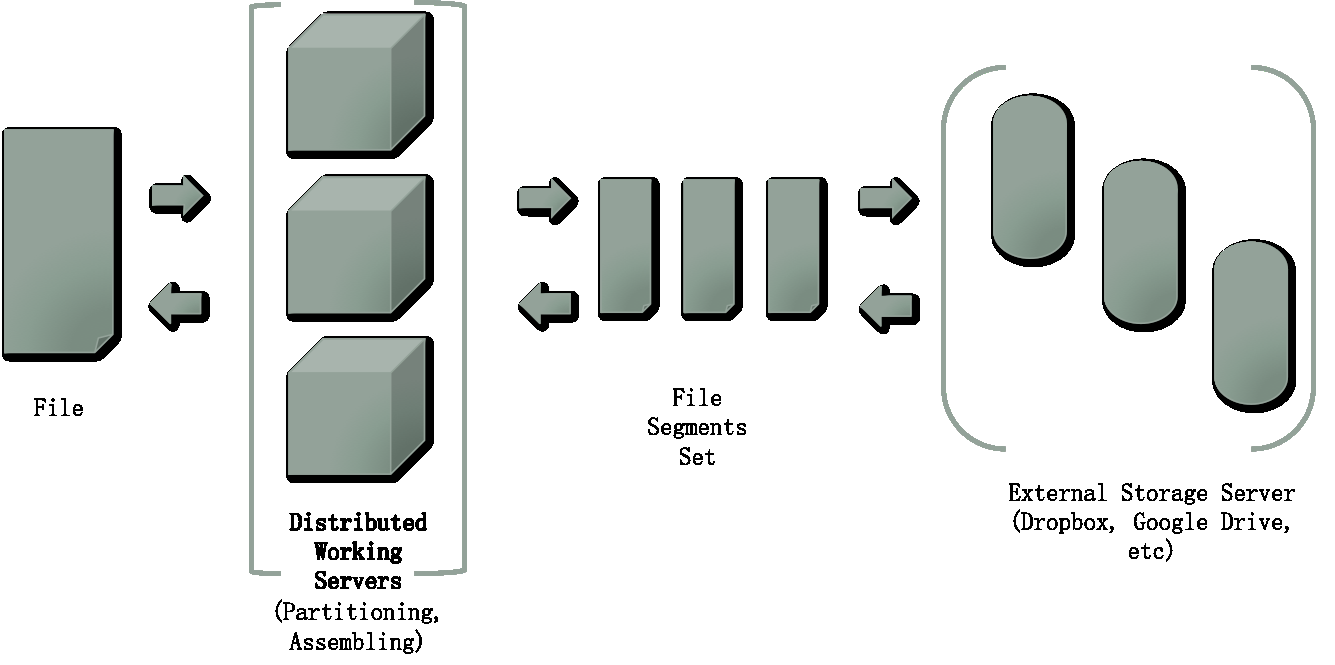
\includegraphics[width=6.5in]{pics/system_architecture-eps-converted-to.pdf}
\caption{Framework}
\label{fig:frame}
\end{figure*}

\subsubsection{Client}
The system (distributed working servers) provide users with uploading, downloading, deleting, newing folders, moving data opeations. Especially for the uploading operation usage, the user is required to set the "black-box" key and specified the security level {normal, high, premium} (higher level means more fragments a file will be partitioned, and it would lead to more time to process), which can be a figure or any combination of string and digits.Besides, the user need give the system access privilege to the external cloud storage servers (Google Drive, SkyDrive, Dropbox, etc). System will automatically maintain a table to record all the files' names and indices of their corresponding partitioned fragments. 

\subsubsection{Server}
Server need be in charge of three responsibilies: determining how to partition the file based on the key given by the user and carrying out the work, communicating with clients and external cloud stroage by transferring kinds of data, assembling the fragments to the original file. In the server, it needs update a dictionary to store which storage server the fragment has been stored and maintains the encrypted version of users' table.
The system still need perform a "heart-beat" function to update this encrypted table by communicating with users periodically.
\subsubsection{External distributed server}
External distrbuted storage servers provide interface to working servers. They are responsible for storing, replicating, backup files.


\section{Software Artifact}
We build a system contains as follows, 

%1. The particular software artifact to complete:

(1) A web interface for user to upload, download files and create folders, etc, like the functionality Dropbox website provides.
When initializing his/her account, the user can choose the security level and integrate with his/her third-party cloud storage platforms.


(2) A server-side distributed files system to handle the file partitioning and assembling, using API from
% Google Drive, 
Dropbox to utilize their services. 
When user uploads a file, our server help partition (or encrypt if the security level is premium) this file, and perform as a \emph{bridge} between
the user and third-party cloud storage server. %to differen 
When user want to fetch a file, it invokes our server-side program to fetch the files fragment from different storage hosts and assemble them into the original file.
The methodology is given in~\ref{sec:approach}.
The blue parts of Fig. \ref{fig:arch} and Fig \ref{fig:web} are built by us.
\begin{comment}
2. A high-level description of the design of your system.

See the section \ref{sec:approach}.

3. Any existing software packages you are using as a basis for your development.

Re-use the Tribble code~\cite{CSE230} with Thrift~\cite{thrift} for interaction with clients (trigger the file transfer), 
Tribble Server (Server in our case, to do the hash and file partitioning, also 
handle the file assembling and respond to users) and 
Backend Storage (invoke API to do the real disk storage). 

We will use the API from Google Drive~\cite{googledriveapi}
and Dropbox~\cite{dropboxapi}.

% We also will use XtremeFS~\cite{xtreemfs} to manage the file partioning and asembling table replication and storage in our server. 

4. Your evaluation plan for this artifact. How will you measure success? What will you use for a testbed? Do you need any resources from us?

For the upload partition of file, in Google Drive and Dropbox, etc, we will dectect the file fragments. When you click the third-party, you cannot see the whole file,
and the third-party cannot recover the file among these unordered fragments.

For fetching a file, the correctness should be gauranteed, it is easy to check to ``diff'' the original file and download file.

The efficiency is the tradeoff with the granularity (security). If user choose large granularity, which will bring more efficiency for partioning or assembling, but less security.
\end{comment}
 


 
\section{Implementmentation}

\subsection{System Architecture}

\begin{figure*}[ht]
\centering
%\includegraphics[width=3.5in]{pics/system_architecture.eps}
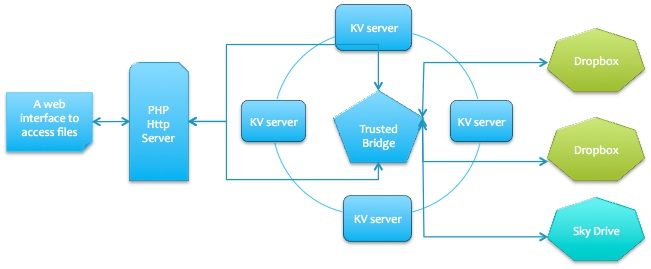
\includegraphics[width=5.2in]{pics/arch.png}
\caption{Trusted Bridge architecture}
\label{fig:arch}
\end{figure*}

Trusted Bridge provides users a convenient online storage environment without losing their privacy. To achieve this goal, we implement the system with the following structure, please see Figure~\ref{fig:arch}. We build all the blocks with blue color and take advantage from lab3 key-value storage system. The Trusted Bridge server and key-value storage server are built in sysnet clusters. The front-end web server is portable. It could be served right into sysnet clusters but it also could be run as a remote service on any Apache and PHP environment. The following sections will describe the detail implementation of each components. 




\subsection{Front-end Web Server}

\begin{figure*}[ht]
\centering
%\includegraphics[width=3.5in]{pics/system_architecture.eps}
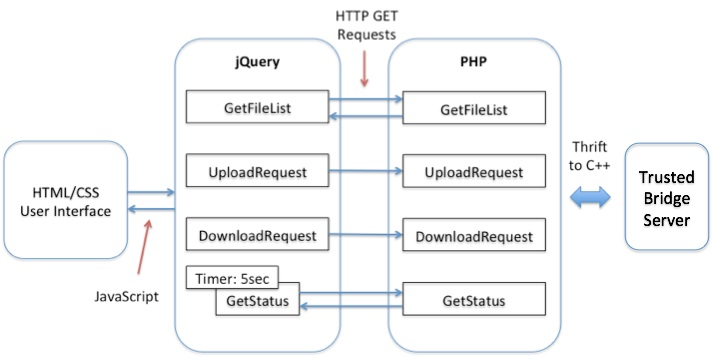
\includegraphics[width=5.2in]{pics/web_arch.png}
\caption{Front-end web server architecture.}
\label{fig:web}
\end{figure*}

Trusted Bridge has an elegant web user interface to provide the user with an intuitive click-and-go file upload and download accessibility. The front-end web service is composed of three
components: HTML/CSS for the interface template, JavaScript/jQuery for UI logic control, and PHP for handling file upload and download from client browsers. Figure~\ref{fig:web} shows the architecture of the front-end web server.

We use Twitter Bootstrap to rapidly build the web user interface. Bootstrap contains HTML and CSS-based design templates for typography, forms, buttons, navigation and other interface components, as well as some useful JavaScript extensions. The HTML/CSS contents will be automatically updated to reflect the current system status including the error message from Trusted Bridge server, the change of file list, upload and download progress, and etc. 

With the help of jQuery, we could easily modify the HTML/CSS DOM objects dynamically. The UI event will trigger callback functions written in jQuery and do the related action. All the requests will be forwarded to a PHP program, which could arbitrarily access files on web server with appropriate permissions. The PHP program will talk to Trusted Bridge server through Apache Thrift protocol.

For example, when the user click on "Add File" button, a file selector will pop out. After the file selection by the user, the file upload event in jQuery will be triggered and send the selected file from user's local storage to web server temporary folder. The PHP program will handle the upload request and send the file location to Trusted Bridge server. After the file partitioning and uploading to external cloud storage, Trusted Bridge server will response a OK message. The PHP program will just pass this response to front-end JavaScript with JSON format. When the front-end get the response, it will call GetFileList to get the latest file list in the system.

For downloading files, when the user click on the download button right next to the file name, jQuery will send a HTTP request to PHP server to ask for download action. The PHP program then forward the request to Trusted Bridge server through Thrift. After the file assembling task is finished, a downloadable intact will be saved in web server temporary folder. The front-end jQuery will check whether the file is ready or not every five seconds with the help of PHP server. Once the file is ready, the requested file will be automatically downloaded into user's local disk.



\subsection{File Partition and Assembling}


File Partitioning is the key point of this system and it inclues two main 
problems: first one is how to partition the file and the 
other one is how fine-grained the file need to be partitioned.
For the first one, 
when a file is uploaded to our server, we need to dispatch the file to different
cloud storages. Our strategy is to read the 
file and truncate content on the fly, so that
the large files do not occupy the large chunk of memory.
For implementation, we also use JSON in Boost to  
control hierachical key value format, e.g. the order of segments for a file,
the mapping from file to segments and different cloud services.
First, the process get the parameter vector to specify how many segments for this
file, and what the sizes are respectively.
During the processs of spliting, it also invokes \emph{GetSegmentName()} to get a 
encrypted name for such segement, which appear in the cloud storage. Others cannot 
judge the file by name. The method of \emph{GetSegmentName()} is demonstrated in Sec. \ref{naming_hash}.
The pseudo code is shown in Fig. \ref{fig:fsplit}.

%\setlength{\belowcaptionskip}{0pt minus 10pt}
\begin{figure*}[hbt]
\centering
\begin{lstlisting}
fp = fopen(file, "rb"):
for (int it = 0 ; it < chunk_size_array.size ; it++){
  buffer = malloc(chunk_size_array[it]);
  file_name = GetSegmentName(user_key)
  // treating every file as binary 
  segment_file = fopen(file_name, "wb")
  fwrite(buffer,1,current , segment_file);
  fclose(segment_file);
  free(buffer);
  // use hierachical Key Value pair by JSON 
  // It provide a file contains what segments,
  // their order, and position.
  // Simplify the process by register_to_key_value() as follows
  register_to_key_value(user, cloudID, file , segment_order , segment_name);
}
\end{lstlisting}
\caption{Pesudo Code of File Spliting}
\label{fig:fsplit}
\end{figure*}

For the merge of segments from different clouds, we fetch them from their repositories at first, 
Following the records from our key value storage, assemble them together accordingly.

\begin{comment}
\begin{figure}
\centering
\begin{lstlisting}
// Download the segments in order througth Key Value storage's guide
std::list<string> l;
int index = 1;
BOOST_FOREACH(ptree::value_type& v, pt.get_child("array")){
   counter = boost::lexical_cast<string>(index++);
   segmentName = v.second.get_child(counter).data();
   key = FormKey(user_key, segmentName);
   GetResponse response = Get(key);
   // find out which cload ID
   extid = response.value;
   Download(username, segmentName, cloudID);
   l.push_back(segmentName);    
}

file_name
fp = fopen(file, "rb"):
for (int it = 0 ; it < chunk_size_array.size ; i++){
  buffer = malloc(chunk_size_array[it]);
  file_name = GetSegmentName(user_key)
  // treating every file as binary 
  segment_file = fopen(file_name, "wb")
  fwrite(buffer,1,current , segment_file);
  fclose(segment_file);
  free(buffer);
  // use hierachical Key Value pair by JSON 
  register_to_key_value(user, file , segment_order , segment_name);
}
\end{lstlisting}
\caption{Pesudo Code of File Merge}
\end{figure}
\end{comment}



\begin{figure*}
\centering
\begin{lstlisting}
    key                                 Value
    ---------------------------------------------------
    ${username}_clouds             (JSON) clouds
    ${username}_files              list<filename>
    ${username}_${filename}        list<segment_name>
    ${username}_${segment_name}    cloud_id
    ${username}_key                any string
    ---------------------------------------------------
\end{lstlisting}
\caption{Key-Value Storage Format}
\label{fig:kv_format}
\end{figure*}


\begin{figure*}
\centering
\begin{lstlisting}
	    early_cloud  {
	    "clouds":[
	    {"id":0, "type":"dropbox", "token1":"12345",  "token2":"67890" },
	    {"id":1, "type":"dropbox", "token1":"12345",  "token2":"67890"},
	    {"id":2, "type":"google" , "token1":"12345",  "token2":"67890"}
	    ]
	    }
	    early_files             list<"file1.avi","file2.txt","file3.jpg"...>
	    early_file1.avi         list<"seg1.seg","seg2.seg","seg3.seg"...>
	    early_file2.txt         list<"seg1.seg","seg2.seg","seg3.seg"...>
	    early_seg1.seg          0
	    early_seg2.seg          1
	    early_seg3.seg          2
\end{lstlisting}
\caption{Example of Our Key Value Pair}
\label{fig:example-kv}
\end{figure*}
																																																																																																																																									      







\subsection{Segment Naming, and Ordering}
\label{naming_hash}
%\subsubsection{Hash Function}
A hash functin is to transform an arbitray set of data elements, such as a text file into a single fixe length value (the hash). Its main advantage is the computed hash value may then be used to verify the integerity of copies of the original data without providing any means to derive said original data. We want a strong hash function (without collision) to generate a unique hash value for each arbitrary set of data. SHA-2 is a set of cryptographic strong hash functions that can prevent the exposed attack on SHA1 family hash algorithms.So in this system we adopt SHA2-256 algorithm in the SHA2-family hash function. SHA2-256 can transfer any data into fixed 32bytes length hash value.

\subsubsection{File Segment}
Our system need a "black-box" key to generate the hash value to determine how to partition the file into fragments. Each time a new account has been created and then this "black-box" key is required to be created by the user. E.g, the "black-box" key is "ucsd" and the corresponding hash value is "0x 8c:f3:95:33:75:84....". We let each two hexical value as a group so that each SHA2-256 hash value can support 32 groups. For each group g(i), we take the method that add the two hexical values together (e.g. Ox8c represents 0x8 + 0xC = 20) and divide it by the sum of each digits (e.g. 20+18+...)in the hash value to determine how much percentage of file fragment f(i) will take. In this way, we are going to partition a file into 32 fragments at most. Next Step is to calculate the actual size of each fragment shall hold, a straightforward way is to multiple the size of one document by the percentage of each document fragment. As all the fragments are generated, we assign the filename for each document with the hash value of itself. A table for each document called file\_Structure\_index is used to record all the filenames belongs to it.   





%\subsubsection{Segment Name and Ordering}

As each file can be partitioned into 32 segments or more, to make segment name unique comes to be a problem. Because we do not want any file to be overwritten. 
The other question is to maintain the generating ordering of segments, which is used to assemble the file. Any small mistake here will results in failing in recovering the original file. For the first question, two conditions shall meet: first one is segment name shall be unique, sencond is that the name shall be random. SHA2-256 provide sufficient functionality that different input always gives out different hash value, which can satisfy our first condition. For the second one, we at the beginning adopt the method to give a random number among a pretty large range. After several experiments on random number generating, due to the bad distributuion of random number, some number will be generated the same in the second time. Then we change the strategy to take the system CPU counter as the input that always is unique as the seed of hash function. In this way, we first get the system CPU counter and get the corresponding unique hash value, later this will act as the name of segment.

Segment Ordering provides the mapping structure when assembling the file. This requires a stable data structure or some other kinds of format maintaing the segment generating order. Each time we get a new segment, a new item as talked above is enqueued to the uploading task queue with counter for this queue. As soon as the item successfully gets into it, a key$-$value pair $<$segment name, counter$>$ (segment with counter i means it is the i-th part of the file). Till finish partitioning file into segments, we collect all of these pairs as json array into the json object whose key is the name of the file. When trusted bridege server want resemble file, it is straigtforwatd to get the order of segment by parsing the json object by given the file name.

\subsection{Key-Value strucutures}
To provide more convenient service for trusted bridge server, 
we design the following key value pairs. 
The first kind $<$username clouds, token array for the cloud storage$>$ 
is used to record user's tokens for different cloud storage access. 
The second kind $<$username files , filename lists$>$ record the list 
of filenames the user has uploaded. 
The key for the third one is username plus filename,
the value corresponding to it is the list of segment name. 
The fifth pair's key is username plus segment name, 
the value is the place of the cloud who has this segment. 
The last kind is the pair username and the key it specified 
when registraing a new user. 



\section{Evaluations}
\label{sec:exp_results} 

\subsection{Measurement Method}
To get more accurate performance measurement result, we design the experiment very carefully. First, we assume that Dropbox API will compare user data with what the already had in the cloud before the API actually upload the file. It is reasonable for them to do so to avoid massive redundant uploading bandwidth. However, for our measurement, this is not a good property because the upload speed will be much faster than it should be after the first upload action. To avoid this kind of situation, we generate a new random file with a random file name from system random source /dev/urandom each time before we upload it. Since each time both the file name and the content is different, the Dropbox API has no chance to compare the data before upload. Then we can measure the actual time consuming during upload/download progress.

Second, as the suggestion from Professor Alex C. Snoeren, we also scramble the order of uploading and downloading tasks. Sequential uploading or downloading files with the same file size could not ignore the fact that the network between sysnet clusters and Dropbox is not always stable. The file-transfer-speed statistics collected could be affected by the current network condition. We generate a random test order for different file size to avoid this problem. In the following evaluation, we run each test at least 100 times and get the average data from the results.

Third, we run the test with different Dropbox accounts and different sysnet cluster machines. Keep running a script that uploads and downloads small files continuously maybe will soon be noticed by Dropbox servers. To avoid the possible limitation on file-transfer-speed by the service providers, we switch the account randomly and test the script on different machines with different IP address.

\subsection{Dropbox Overhead and Performance}
We first found that the Dropbox Java API has a huge overhead on each uploading and downloading operation. This overhead dramatically slows down the performance of Trusted Bridge. We do not have enough time to implement the API by pure HTTP requests, so we decide to test the Dropbox API overhead and assume that we could minimize this overhead in the future with better implementation. The method to estimate the overhead is to generate a empty file by linux touch command. The file will be created with 0 Byte disk occupation and online contains metadata information. The average upload time for one single upload task with one empty file is 3.45 seconds. The average download time for the same file just uploaded is 3.12 second. 

To test the general performance of Dropbox uploading and downloading performance, we generate a series of random files with size 1Byte, 1KB, ad 1MB to 128MB. The result is shown in Figure~\ref{fig:dropbox_speed}. All the statistics are in Mbps unit. Averagely the download speed is a little faster than upload speed. The difference is about 3Mbps, which is not so significant. The interesting fact here is the performance is very bad when uploading or downloading small files. The speed is converged at about file size 4M to 8M. According to this phenomenon, we believe that Dropbox API will do file upload and download in chunk. The chunk size should be around 4M to 8M. 

\begin{figure}[ht]
\centering
%\includegraphics[width=3.5in]{pics/system_architecture.eps}
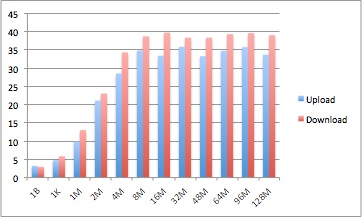
\includegraphics[width=3.5in]{pics/dropbox_speed.png}
\caption{Dropbox upload and download performance}
\label{fig:dropbox_speed}
\end{figure}

\subsection{Trusted Bridge Performance}
Figure~\ref{fig:upload_line} shows the upload speed comparison between Dropbox and Trusted Bridge server. The performance of Trusted Bridge on uploading small files are significantly worse than using pure Dropbox API. Figure~\ref{fig:download_line} shows the download speed comparison. Very similar pattern is showed in the graph as uploading test. The best performance lose is 9.57\% with the file size 128M. The worst performance lose for uploading, however, is 97\% with file size smaller than 4M. The best performance lose is 8.62\% with the file size 128M. The worst performance lose for uploading, however, is 96\% with file size smaller than 4M. 

The main reason of the performance degradation is that we separate each uploaded files into 32 pieces and upload them through Dropbox API one by one. The Dropbox API overhead will dramatically affect on our system performance. We believe we could find a better way to handle external cloud storage, so here we assume that we could remove the effect of the Dropbox uploading and downloading overhead. Because each file needs 32 upload or download task, we compare the speed performance between Trusted Bridge and Dropbox uploading or downloading the same actual file size. For example, uploading 128M file to Trusted Bridge server compare to uploading 4M file to Dropbox. The result is shown in Figure~\ref{fig:upload_bar} and Figure~\ref{fig:download_bar}. In this comparison, we could found that Trusted Bridge server only lose averagely 8.2\% on uploading and 9.7\% on downloading speed. This result shows the overall partitioning and assembling performance do not degrade the system performance too much. With our robust file scrambling algorithm, the user could save their files in their own cloud storage without losing the privacy. What he or she scarifies is just about 8 to 10 percent performance lose, which could hardly be noticed especially when user run our service in background like how current Dropbox or Google Drive works.


\begin{figure}[ht]
\centering
%\includegraphics[width=3.5in]{pics/system_architecture.eps}
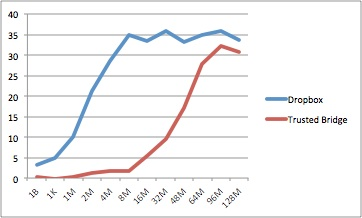
\includegraphics[width=3.5in]{pics/upload_line.png}
\caption{Upload speed comparison}
\label{fig:upload_line}
\end{figure}

\begin{figure}[ht]
\centering
%\includegraphics[width=3.5in]{pics/system_architecture.eps}
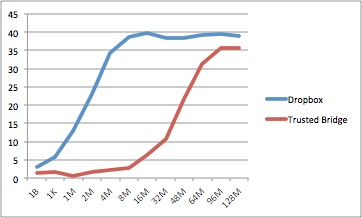
\includegraphics[width=3.5in]{pics/download_line.png}
\caption{Download speed comparison}
\label{fig:download_line}
\end{figure}

\begin{figure}[ht]
\centering
%\includegraphics[width=3.5in]{pics/system_architecture.eps}
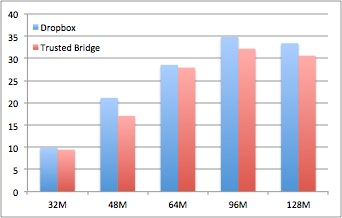
\includegraphics[width=3.5in]{pics/upload_bar.png}
\caption{Calibrated upload speed comparison. The file size here is the size uploaded to Trusted BRidge server}
\label{fig:upload_bar}
\end{figure}

\begin{figure}[ht]
\centering
%\includegraphics[width=3.5in]{pics/system_architecture.eps}
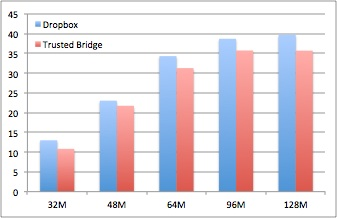
\includegraphics[width=3.5in]{pics/download_bar.png}
\caption{Calibrated download speed comparison. The file size here is the size downloaded from Trusted BRidge server}
\label{fig:download_bar}
\end{figure}



\section{Discussion and Future Work}
\subsection{Upload Task Queue}

As each file would be partitioned into 32 or more segments and then they shall be pushed to external kinds of cloud storage servers, we take this way to loosely separate these two kinds of work. The main thread of trusted bridege server still take the responsibility for generating the segments. The reason why we just use one thread here is to decrease the possibility of erronously partitioning the file. Consider that several threads are working for generating new segments, shared lock for the file need be maintained for synchronizing reading the file. This will lead to a high overhead. What's worse is when a thread crashed, the segment it's responsible for will be abnorammly generated or some other kinds of errors may happen. If so, it will violates the most imporant part for trusted bridge server, what is to store complete information about the file and related segments. While, the independent segments generated by trusted bridege server can be severd with sveral threads. 
When initializing the trusted bridge server, there threads are created for dealing with the segment uploading task. A one\-writerr\-more\-reader task uploading queue will be created as the working pool for trusted bridge server. This queue maintains one mutex and one condition variiable for threads sharing. When going into "enque" opeartion, the thread need first acquire the mutex for this queue, if it's permitted, one new entry that contains the pair <username, segment name, cloud id to store current segment> is pushed back to the queue, meanwhile, \"notify\-to\-one\" for the condition variable is called to wake the thread waiting for new segment. If this queue is full, resize opeartion will be invoked. For "deque" operation, the mutex still need be checked firstly. Simiarly, it gets the access if allowed and then check segment ready for being uploaded. If there exists one, the item records the uploading specification will be removed from the queue and be transfereed to uploadToServer function. 


\subsection{Fault-Tolerance Scheme}
%\subsection{Fault Tolerance}
Two big issues here need be more focused. One is that we cannot lose anything about the mapping strucuture between file and related segments. We solve this by using a replicated key value distributed storage server. As one trusted bridge server just talks to one key value storage server one moment in time, the replicated storage server will help syncrhonize writing key value pair by communicating with each other in order to prevent some storage server crashing. This method will enormously get the risk out. 
The second one is to keep data consistent during the period of generating the segment. For example, server may fail in trasmitting segments to the cloud. To fix this, a thrad can be used to monitor and periodically check whether the segment has been put on the external cloud storage. If it has been there, the server begin to update the item to array in the mapping structure for this segment. If it is not, the trustd bridge server shall resend current current segment. When learning that all the segments for one file have been pushed to the cloud, the json object describing one file with corresponding segments will be put into the key value storage server. The user will not get the information that the file has been uploaded successfully till we get the commit acknowledgement from the key value storage server.


\subsection{Text Mining}

Text mining methods, there is no major increased computational complexity when analyzing many short documents, compared to the same number of words in fewer documents.A much more important issue is whether individual documents are well-defined in a meaningful way. Most text mining methods work best on documents whose length is a paragraph to a page. Too short documents like tweets cannot be understood well without context. Too long documents like books lack homogeneity and need to be divided into segments. The more segments the file is divided, the more diffculty will put on the analyzers. Take the TF(term frequency)-IDF(Inverted Document Frequency) algorithm to weight the keywords for a file as an example. The partitioning will change the term frequency for keywords, which will definitely change each keyword's weight. Besides, as we distributed segments to different servers, the IDF value would still change. Because these two values are changing together, it will direct user the wrong way analyzing the file, which is the target trusted bridge server want serve.


%\subsection{Synchronization to Asynchronization}
%
sync

use one-way RPC


\subsection{Programming Language Integration}
In this implementation, we totally use at least four different programming language including HTML/CSS/JavaScript, PHP, C/C++, and Java. That was because we first write our Trusted Bridge server in C/C++ as an extension of lab3 key-value storage system. C/C++ is powerful and efficient, but it lacks cloud storage API support and HTTP request handler. The difference of programing environment slows down the development progress and the system could not take advantage from compiler level memory and CPU optimization. If we have the opportunity to redesign this system, we would like to rewrite Trusted Bridge server in Java, and the dynamic web server in JavaServer Pages (JSP). In this case, Trusted Bridge could be integrated with Dropbox or Google Drive API in JAVA much more closely. The front-end server also could talk to Java Servelet directly without the Thrift protocol overhead. The new system could be implemented with HTML/CSS/JavaScript, JSP, and Java, which is much more easy to maintain and much more efficient. 


%%%%%%%%%%%%%%%%%%%%%%%%%%%%
\section{Conclusion}
\label{sec:conclusion}
In this project, we derive our own idea and build a trustful file system
\emph{Trusted Bridge}, which utlizes unstrustful popular cloud storages, e.g. Dropbox.%, Google Drive. 
% We treat them as a untrusted storage systems, so that we build a bridge to  
The approach is to partition the files, encrypt, and then send them into different cloud systems. 
% We do not save users' files on our Trusted Bridge, while the other cloud storages 
% only contains the segements of a single file.
For a single file, we do not save it, and the cloud storages only contains a certain part of file 
segments. 
In this project, we use C/C++ to handle the backend design and use wrap interface to invoke Jave, Python
for API from Dropbox, Google Drive. The PHP is used to handle the HTTP requests. 
Experiement shows that after removing the Dropbox API overhead, the user could save their files in their own cloud storage without losing the privacy. What he or she scarifies is just about 8\% to 10\% performance lose, which could hardly be noticed especially when user run our service in background like how current Dropbox or Google Drive works.





\bibliographystyle{abbrv}

\bibliography{paper}  


\section{Appendix}

In the appendix, we provide a snapshot of the code to further utilize
multi-thread environment and speedup backend for handling the file uploading and downloading.
There are Locking Queue and corresponding Pthread programming, which are discussed in
\ref{naming_hash}
.


\subsection{Locking Queue}
The locking queue class for future usage. 

%\begin{figure}[h]
%\centering
\begin{lstlisting}
template <typename Data>
class oncurrent_Queue{
private:
    queue<Data> _queue;
    mutable boost::mutex _mutex;
    boost::condition_variable _cvariable;
public:
    void enque(Data const& data){
	boost::mutex::scoped_lock lock(_mutex);
	_queue.push(data);
	lock.unlock();
	_cvariable.notify_one();    
    }

    bool empty() const{
	boost::mutex::scoped_lock lock(_mutex);
	return _queue.empty();    
    }

    bool try_deque(Data& dequed_value){
	boost::mutex::scoped_lock lock(_mutex);
	if (_queue.empty()){
	    return false;
	}    
	dequed_value = _queue.front();
	_queue.pop();
	return true;
    }

    void wait_and_deque(Data& dequed_value){
	boost::mutex::scoped_lock lock(_mutex);
	while(_queue.empty()) _cvariable.wait(lock);
	dequed_value = _queue.front();
	_queue.pop();    
    }


};

void *checkUploadQueue(void* context){
    int id = *(int*)thread;
    while(true){
	if (!uploadQueue.empty()){               
	    string ret;
	    uploadQueue.try_deque(ret);
	}
    }
}
\end{lstlisting}
%\end{figure}

\subsection{Pthread}

The pthread can be utilized to 
listen to the upload queue.

%\begin{figure}[h]
\begin{lstlisting}
  TrustedBridgeHandler t(storageServer, storageServerPort);
  const int NUM_UPLOAD_THREADS = 3;
  pthread_t threads[NUM_UPLOAD_THREADS];;
  for (int i = 0; i < NUM_UPLOAD_THREADS; ++i){ 
      int rc = pthread_create(&threads[i], NULL, &TrustedBridgeHandler::checkUploadQueue, &t);
      if (rc){
	  exit(-1);    
      }    
  }
\end{lstlisting}
%\end{figure}



% sigproc.bib is the name of the Bibliography in this case

% Can use something like this to put references on a page
% by themselves when using endfloat and the captionsoff option.
\ifCLASSOPTIONcaptionsoff
  \newpage
\fi



% trigger a \newpage just before the given reference
% number - used to balance the columns on the last page
% adjust value as needed - may need to be readjusted if
% the document is modified later
%\IEEEtriggeratref{8}
% The "triggered" command can be changed if desired:
%\IEEEtriggercmd{\enlargethispage{-5in}}

% references section

% can use a bibliography generated by BibTeX as a .bbl file
% BibTeX documentation can be easily obtained at:
% http://www.ctan.org/tex-archive/biblio/bibtex/contrib/doc/
% The IEEEtran BibTeX style support page is at:
% http://www.michaelshell.org/tex/ieeetran/bibtex/
%\bibliographystyle{IEEEtran}
% argument is your BibTeX string definitions and bibliography database(s)
%\bibliography{IEEEabrv,../bib/paper}
%
% <OR> manually copy in the resultant .bbl file
% set second argument of \begin to the number of references
% (used to reserve space for the reference number labels box)

% biography section
% 
% If you have an EPS/PDF photo (graphicx package needed) extra braces are
% needed around the contents of the optional argument to biography to prevent
% the LaTeX parser from getting confused when it sees the complicated
% \includegraphics command within an optional argument. (You could create
% your own custom macro containing the \includegraphics command to make things
% simpler here.)
%\begin{IEEEbiography}[{\includegraphics[width=1in,height=1.25in,clip,keepaspectratio]{mshell}}]{Michael Shell}
% or if you just want to reserve a space for a photo:

 

% You can push biographies down or up by placing
% a \vfill before or after them. The appropriate
% use of \vfill depends on what kind of text is
% on the last page and whether or not the columns
% are being equalized.

%\vfill

% Can be used to pull up biographies so that the bottom of the last one
% is flush with the other column.
%\enlargethispage{-5in}



% that's all folks
\end{document}


